\chapter{积分变换法}
\intro{本章介绍利用傅里叶变换和拉普拉斯变换求解 PDE 的方法。}

\section{傅里叶变换法}

\begin{mydefinition}{傅里叶变换}
\[
\hat{f}(\omega)=\mathcal{F}[f]=\int_{-\infty}^{+\infty}f(x)e^{-i\omega x}\,dx
\]
逆变换：
\[
f(x)=\mathcal{F}^{-1}[\hat{f}]=\frac{1}{2\pi}\int_{-\infty}^{+\infty}\hat{f}(\omega)e^{i\omega x}\,d\omega
\]
\end{mydefinition}

\begin{theorem}[导数的傅里叶变换]
$\mathcal{F}[f^{(n)}]=(i\omega)^n\hat{f}(\omega)$
\end{theorem}

\begin{remark}
傅里叶变换将微分运算转化为乘法运算，将 PDE 转化为关于时间的 ODE。
\end{remark}

\section{拉普拉斯变换法}

\begin{mydefinition}{拉普拉斯变换}
\[
F(s)=\mathcal{L}[f(t)]=\int_0^{+\infty}f(t)e^{-st}\,dt
\]
\end{mydefinition}

\begin{theorem}[微分性质]
\begin{align*}
\mathcal{L}[f'(t)]&=sF(s)-f(0)\\
\mathcal{L}[f''(t)]&=s^2F(s)-sf(0)-f'(0)
\end{align*}
\end{theorem}

\begin{figure}[htbp]
\centering
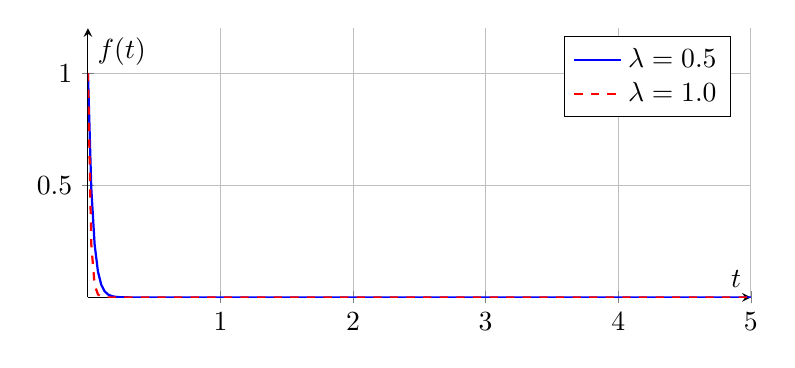
\begin{tikzpicture}
\begin{axis}[
	axis lines=middle,
	xlabel=$t$,
	ylabel={$f(t)$},
	xmin=0,xmax=5,
	ymin=0,ymax=1.2,
	legend pos=north east,
	grid=major,
	width=10cm,height=5cm,
]
\addplot[blue,thick,domain=0:5,samples=200]{exp(-deg(x)*0.5)};
\addplot[red,dashed,thick,domain=0:5,samples=200]{exp(-deg(x)*1.0)};
\legend{$\lambda=0.5$,$\lambda=1.0$}
\end{axis}
\end{tikzpicture}
\caption{指数衰减}
\end{figure}

\begin{remark}
拉普拉斯变换适用于半无界问题（$x\in[0,+\infty)$），傅里叶变换适用于全空间问题。
\end{remark}
